\section{Topological Manifolds}

\begin{definition}
    A \textbf{topological $n$-manifold} is a second countable Hausdorff space
    $M$, together with a collection  $\{(M_\a,\phi_\a)\}$ for which
    \begin{enumerate}
        \item[(1)] $\{M_\a\}$ is a collection of open sets of $M$ covering $M$ ;
            that is, $M_\a \subseteq M$ is open and  $M=\biogcup{M_\a}$.

        \item[(2)] $\phi_a$ is a homeomorphism of  $M_\a$ onto an open subset
            $U$ of  $\R^n$.
    \end{enumerate}
    We call the pairs $(M_\a,\phi_\a)$ \textbf{charts} of $M$, and we call the
    collection of all such charts of $M$ an  \textbf{atlas} of $M$. We define
    the  \textbf{dimension} of $M$ to be  $\dim{M}=n$.
\end{definition}

\begin{example}\label{example_1.1}
    \begin{enumerate}
        \item[(1)] Every subset of $\R^N$ is second countable and Hausdorff, so
            that a subset  $\R^N$ is an  $n$-manifold uf every point of  $M$ has
            a neighborhood homeomorphic to  $\R^n$, for $n \leq N$. In
            particular, $\R^n$ is an $n$-manifold.

            \item[(2)] The $n$-sphere  $S^n=\{x \in \R^{n+1} : \|x\|=1\}$ (see
                figure \ref{fig_1.1}) is an $n$-manifold. It is a second countable
                Hausdorff space, since it is a subspace of  $\R^n$. Moreover, the
                stereographic projection $h:\com{S^n}{(0, \dots, 0,1)}
                \xrightarrow{} \R^n$ is a homeomrphism. So for $x \in S^n$,
                $x \neq (0, \dots, 0,1)$, $x$ has a neighborhood homeomorphic to
                $\R^n$. Now, if we take the composition of  $\R^n \times \{0\}$
                with $h$ to obtain the map  $h':\com{S^n}{(0,\dots,0,-1)}
                \xrightarrow{} \R^n$, then we get that $\com{S^n}{(0, \dots, 0,-1)}$
                is a neighborhood of $(0, \dots, 0,1)$ homeomorphic to $\R^n$.
                  \begin{figure}[h]
                     \centering
                     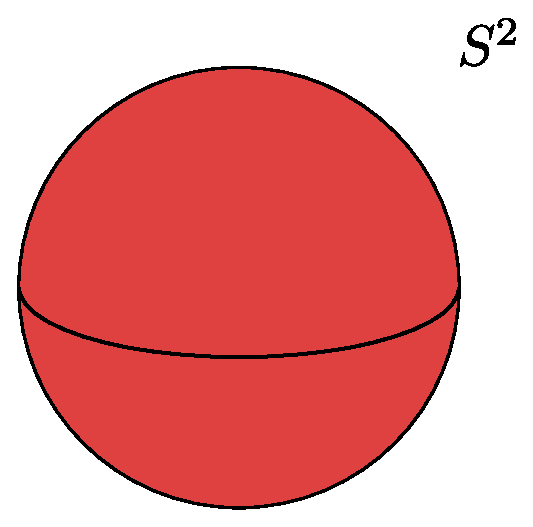
\includegraphics[scale=0.5]{Figures/Chapter1/2_sphere.eps}
                     \caption{The $2$-Sphere of $\R^3$ is a $2$-manifold.}
                     \label{fig_1.1}
                 \end{figure}

             \item[(3)] The $n$-torus  $T=\underbrace{S_1 \times \dots \times
                 S^1}_{n \text{ times }}$ (see figure \ref{fig_1.2}) is the quotient
                 space obtained fron $\R^n$ by identfying two points  $x,y \in \R^n$
                 if, and only if there is some $g \in G$ for which $g(x)=y$,
                 where $G$ is the group generated by all translations by distance
                 $1$ along the coordinate axes.
                 \begin{figure}[h]
                     \centering
                     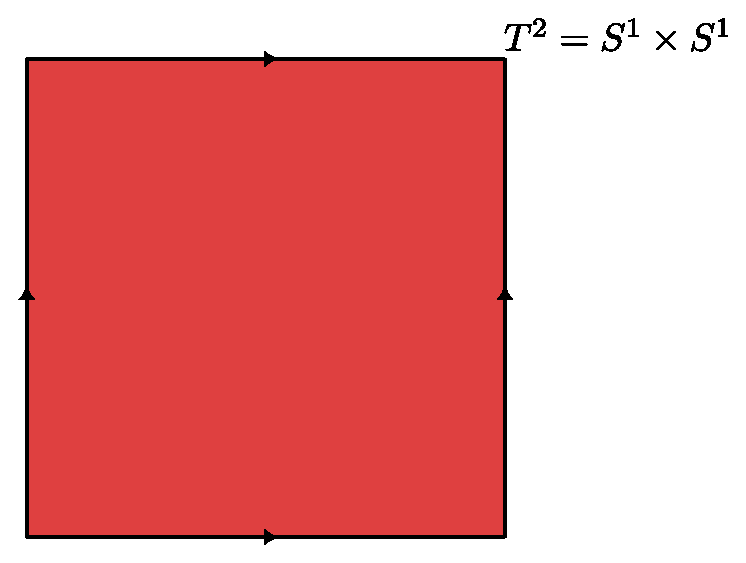
\includegraphics[scale=0.5]{Figures/Chapter1/2_torus.eps}
                     \caption{The $2$-torus is a  $2$ manifold of  $\R^2$.}
                     \label{fig_1.2}
                 \end{figure}
                 Let $x \in T^n$ and  $U=\partial{B(x,\frac{1}{4})}$ the
                 sphere centered about $x$ of radius $\frac{1}{4}$ and let
                 $q:\R^n \xrightarrow{} \R^n$ the quotient map of the quotient
                 space of $T^n$. Then  $\inv{q}|_{q(U)}$ is a homoemorphism.
                 This makes $T$ an  $n$-manifold, with atlas
                 $\{(U,\inv{q}|_{q(U)})\}$.

             \item[(4)] Identify the antipodal points of $S^n$, then the
                 resulting quotient space is an $n$-manifold called
                 \textbf{$n$-dimensional real projective space} which we denote
                 by $\Pb\R^n$. Let $x \in \Pb\R^n$,since $S^n$ is an  $n$-manifold,
                 there is a neighborhood  $U$ of  $x$ and a homeomorphism $h:U
                 \xrightarrow{} \R^n$. Let $-U=a(U)$, where $a:S^n \xrightarrow{}
                 S^n$ is the antipodal map. Then $-U$ is a neighborhood of
                 $-x$, and  $-h=h \circ a$ is a homeomorphism of  $U$ onto
                 $\R^n$. Then the collection  $\{(U,h)\}$ is an atlas for
                 $\Pb\R^n$.

             \item[(5)] Consider the unit circle $S^2$ and the following
                 ``trefoil knot'' $K_3$ pictured below in figure \ref{figure_1.3}
                 \begin{figure}[h]
                     \centering
                     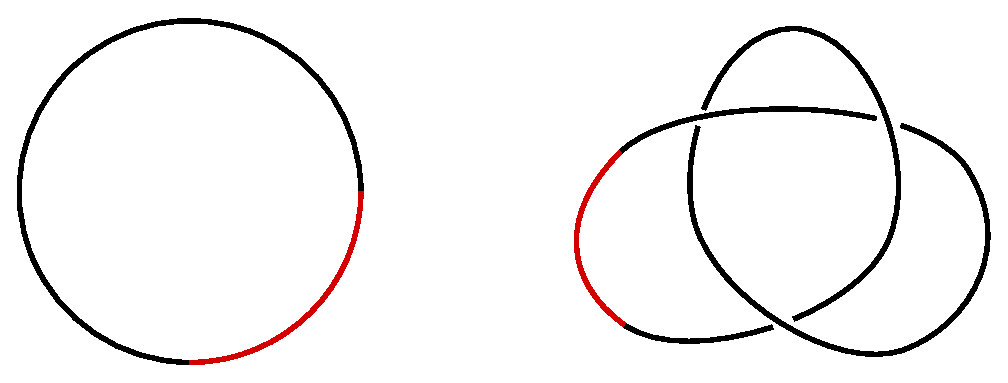
\includegraphics[scale=0.5]{Figures/Chapter1/circle_to_trefoil.eps}
                     \caption{The unit circle $S^2$ and the trefoil knot.}
                     \label{figure_1.3}
                 \end{figure}
                 Both of these are $1$-manifolds, and are homeomorphic to each
                 other. Consider the neighborhoods on either space  (colored in
                 red). Notice that each of these neighborhoods is homeomorphic
                 to an interval in $\R_1$, and hence homeomorphic to each other.
    \end{enumerate}
\end{example}

\begin{definition}
    Let $M$ be an  $n$-dimensional manifold. A  \textbf{$p$-dimensional
    submanifold} of $M$ is a closed subset  $L$ of  $M$ for which there exists
    an atlas  $\{(M_\a,\phi_a)\}$ of $M$ such that for all  $x \in L$, there
    exists a chart  $(M_\a,\phi_\a)$ in where $x \in M_\a$ and  $\phi_\a(L \cap
    M_\a)=\{0\} \times \R^p$.
\end{definition}

\begin{lemma}\label{1.1.1}
    Submanifolds of manifolds are manifolds.
\end{lemma}

\begin{lemma}\label{1.1.2}
    Let $M$ be an  $m$-manifold, and  $N$ an  $n$-manifold. Then the product $M
    \times N$ is an $(n+m)$-manifold.
\end{lemma}
\begin{proof}
    We have that both $M$ and  $N$ are Hausdorff, which makes  $M \times N$
    Hausdorff. Moreover, since  $M$ and  $N$ are second countable, they have
    countable bases  $\Bc_M$ and  $\Bc_N$. Then the product  $\Bc_M \times
    \Bc_N$ serves as a countable basis for  $M \times N$.

    Now, let  $\{(M_\a, \phi_\a)\}$ and $\{(N_\b, \psi_\b)\}$ be atlases for $M$
    and  $N$ respectively. Then since each $M_\a$ is open in  $M$, and each
    $N_\b$ is open in  $N$,  $M_\a \times N_\b$ is open in  $M \times N$.
    Moreover we also have that  $M=\bigcup{M_\a}$, $N=\bigcup{N_\a}$ so that
    \begin{equation*}
        M \times N=(\bigcup{M_\a}) \times (\bigcup{N_\b})=\bigcup{M_\a \times
        N_\b}
    \end{equation*}
    Now, we also have that $\phi_\a$ is a homeomorphism of  $M_\a$ onto an open
    subset of $\R^m$, and  $\psi_\b$ is a homeomorphism of  $N_\b$ onto an open
    subset of  $\R^n$. Since  $\phi_\a$ and  $\psi_\b$ are homeomorphisms, they
    are continuous with continuous inverses  $\inv{\phi_\a}$ and
    $\inv{\psi_\b}$. This makes the map $\phi_\a \times \psi_\b$ continuous with
    continuous inverse $\inv{(\phi_\a \times \psi_b)}$, which makes $\phi_\a
    \times \psi_b$ a homeomorphism of $M_\a \times N_\b$ onto a subset of $\R^m
    \times \R^n \simeq \R^{m+n}$. Therefore $M \times N$ is an
    $(m+n)$-manifold.
\end{proof}

\begin{example}\label{example_1.2}
    The equator, $S^1$ of  $S^2$ is a submanifold of  $S^2$  (see figure
    \ref{fig_1.1}).
\end{example}

\begin{definition}
    We define the \textbf{boundary} of an $n$-manifold $M$ to be the set
    $\partial{M}$, of all points of $M$ for which there is a neigborhood
    homeomorphic to a neighborhood of $H^n$, but no neighborhood homeomorphic to
    a neighborhood of $\R^n$; where $H^n=\{x \in \R^n : x_1 \geq 0\}$.
\end{definition}

\begin{definition}
    Let $H^n=\{(x_1, \dots, x_n) \in \R^n : x_1 \geq 0\}$. We define an
   \textbf{$n$-manifold with boundary}  to be a second countable Hausdorff space
   $M$ with atlas  $\{(M_\a,\phi_\a)\}$ such that $\phi_\a$ is a homeomorphism
   from  $M_\a$ to an open subset of  $\R^n$, or $H^n$.
\end{definition}

\begin{example}\label{example_1.3}
    \begin{enumerate}
        \item[(1)] The unit ball $B^n=\{x \in \R^n : \|x\| \leq 1\}$ is an
            $n$-dimensional manifold with boundary  $\partial{B^n}=S^{n-1}$. For
            interior points of $B^n$, this is clear. For points in  $S^{n-1}$,
            extending the stererographic projection gives the required
            homeomorphism.

        \item[(2)] The \textbf{pair of pants} (see figure \ref{fig_1.3}) Is a
            $2$-manifold with boundary.
             \begin{figure}[h]
                \centering
                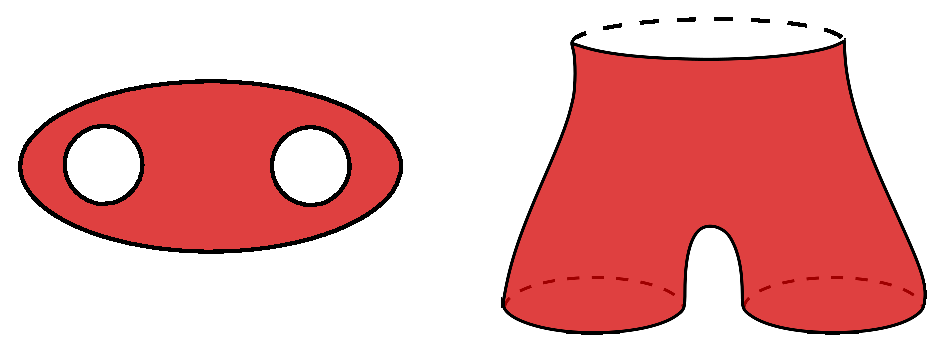
\includegraphics[scale=0.5]{Figures/Chapter1/pair_of_pants.eps}
                \caption{}
                \label{fig_1.3}
            \end{figure}

        \item[(3)] The $1$-holed torus is a  $2$-manifold with boundary.
    \end{enumerate}
\end{example}

\begin{definition}
    A \textbf{$p$-dimensional submanifold with boundary} of an $n$-dimensional
    manifold  $M$ is a closed subset  $L$ of  $M$ for which there is an atlas
    $\{(M_\a,\phi_a)\}$ of $M$ and  $0 \leq p \leq n$, such that for every $x
    \in L$ in the interior of  $M$, there is a chart  $(M_\a,\phi_a)$ such that
    $x \in M_\a$, and  $\phi_\a(L \cap M_\a)=\{0\} \times \R^p$, and for every
    $x \in L$ in the boundary of  $M$, there is a chart  $(M_\a,\phi_\a)$ such
    that $x \in M_\a$, and with  $\phi_\a(L \cap M_\a)=\{0\} \times \R^p$, and
    for which $\phi_\a(x) \in \{0\} \times \partial{H^p}$.
\end{definition}

\begin{lemma}\label{1.1.2}
    The boundary of an $n$-manifold is an $(n-1)$-submanifold with boundary.
\end{lemma}

\begin{example}\label{example.1.4}
    The diameter of the ball $B^2$ is a submanifold with boundary.
\end{example}

\begin{definition}
    We call an $n$-manifold $M$ \textbf{closed} if $M$ is compact with nonempty
    boundary $\partial{M}$.
\end{definition}

\begin{example}\label{example_1.5}
    The $n$-sphere and  $n$-torus are closed manifolds. Additionally, the
    projection map  $\pi_y:T^2 \xrightarrow{} S^1$ fo $T^2=S^1 \times S^1$ onto
    the second factor is a continuous map between manifolds.
\end{example}

\begin{lemma}\label{1.1.4}
    If $M$ is an  $n$-manifold with boundary, then its boundary  $\partial{M}$ is
    an $(n-1)$-manifold without boundary.
\end{lemma}
\begin{proof}
    We first notice by our definition of boundary that $\partial{M} \subseteq M$.
    Since $M$ is second countable and Hausdorff,  $\partial{M}$ inherits these
    properties as a subspace of $M$.

    Now, consider a point $x \in \partial{M}$. Then by definition, there is a
    neighborhood $U$ of  $x$ for which  $U$ is homeomorphic to a neighborhood
    $V$ of $H^n$. Let $\phi:U \xrightarrow{} V$ be the given homeomorphism.
    Notice, that $\partial{H^n} = \{x \in \R^n : x_1=0\}$, and that $\phi(x) \in
    V$ implies $\phi(x) \in V \cap \partial{H^n}$. Since $V$ is open in $H^n$,
    $V \cap \partial{H^n}$ is open in $\partial{H^n}$ as a subspace of $H^n$.
    So that $\phi(U) \simeq V \cap \partial{H^n}$ and $U$ is homeomprphic to an
    open set in  $\partial{H^n}$.

    Now, take the projection map $\pi_y:\partial{H^n} \xrightarrow{} \R^{n-1}$
    onto the second factor, defined by $\pi_y:(0,(x_2, \dots, x_n))
    \xrightarrow{} (x_2, \dots, x_n)=(y_1, \dots, y_{n-1})$. Then $\pi_y$
    defines a homeomorphism of  $\partial{H^n}$ onto $\R^{n-1}$, so that $\pi_y
    \circ \phi$ is a homeomorphism of  $U$ onto an open set of  $\R^{n-1}$. This
    makes $\partial{M}$ an $(n-1)$-manifold. Moreover, since $x \in \partial{M}$
    was arbitrary, there is no $x \in \partial{M}$ with neighborhood
    homeomorphic to an open set in $H^{n-1}$, so that
    $\partial{(\partial{M})}=\emptyset$; i.e. $\partial{M}$ is without boundary.
\end{proof}
